%\documentclass[a4paper,openright,12pt]{book}
%
%\usepackage[utf8]{inputenc}
%\usepackage[spanish]{babel}
%\usepackage{amsmath}
%\usepackage{fancyhdr}
%\usepackage{todonotes}
%\usepackage{graphicx}
%\usepackage{float}
%% aqui definimos el encabezado de las paginas pares e impares.
%%\lhead[Daniel Albendín y ángel Cantó]{Daniel Albendín y ángel Cantó}
%%\chead[]{}
%%\rhead[Resumen]{Resumen}
%%\renewcommand{\headrulewidth}{0.5pt}
%%
%%% aqui definimos el pie de pagina de las paginas pares e impares.
%%\lfoot[Universidad de Huelva]{Universidad de Huelva}
%%\cfoot[\thepage]{\thepage}
%%\rfoot[Proyecto Semandal]{Proyecto Semandal}
%%\renewcommand{\footrulewidth}{0.5pt}
%
%
%
%% Este es un comentario, no será mostrado en el documento final.
%\begin{document}

\chapter{Android}
Android es un sistema operativo basado en el núcleo Linux. Fué diseñado para dispositivos móviles con pantalla táctil. Fue desarrollado por \textit{Android Inc.} empresa que en un principio respaldó Google y terminó comprando  en 2005. Android fue presentado en 2007 con la colaboración de \textbf{Open Handset Alliance}.

Tiene una gran comunidad de desarrolladores de aplicaciones y ha llegado al 1.000.000 de aplicaciones de las cuales dos tercios son gratuitas y más baratas que las mismas en la App Store.

El lenguaje de desarrollo de Android es Java

A la hora de decidirnos por android para desarrollar la aplicación en una plataforma en concreto, hicimos un estudio de mercado y como podemos ver en \href{http://www.xatakandroid.com/mercado/android-se-convierte-en-el-sistema-operativo-movil-mas-usado-de-estados-unidos}{XakataAndroid} Android en 2014 ya superó a iOS en usuarios, por tanto Android al igual que hizo google en su época se está expandiendo y de momento no tiene techo. También podemos ver en la imagen (Ver figura \ref{porcentajesandroid} de la fuente \href{http://www.redusers.com/noticias/navegacion-movil-los-usuarios-de-ios-son-7-veces-mas-activos-que-los-de-android/}{RedUsers} el porcentaje de usuarios de sistemas operativos en dispositivos móviles.


\begin{figure}
\centering
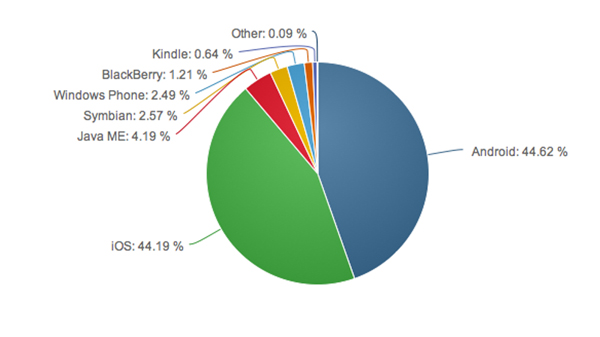
\includegraphics[scale=0.5]{./android/imagenes/porcentaje.jpg}
\caption{Porcentaje de usuarios de los distintos SO móviles}
\label{porcentajesandroid}
\end{figure}




Otro aspecto que hemos tenido en cuenta es la diferencia del desarrollo de aplicaciones para android y para iOS. Es cierto que la programación en android no es algo trivial, pero aun así es más sencilla que en iOS, aunque veríamos satisfechos los frentes de actuación de la aplicación englobando estas dos tecnologías. La implementación en iOS es parte de los trabajos futuros.


\subsection{Aspectos a tener en cuenta}
	\begin{description}
	\item[¿Manejo de base de datos?]
		Realmente en la aplicación de android no viene ningún manejo de las bases de datos propias de la API. Por tanto los datos se obtienen todos por llamadas a ésta. El único manejo de base de datos que debemos saber, únicamente por optimizar tiempos de respuestas y no hacer perder el tiempo al usuario, es SQLite.
	\item[Actividades asíncronas]
		Todas las actividades, tienen dentro su correspondiente actividad asíncrona, es decir, a una clase siempre le corresponde una actividad asíncrona. A continuación explicamos el por qué hemos optado por este tipo de implementación
		\begin{description}
			\item[llamadas a API]
			Como hemos dicho, no manejamos ningún tipo de base de datos externa, y únicamente hacemos uso de las llamada a la API. Una llamada a una dirección web. La gestión de este tipo de llamadas en android debe hacerse en una función asíncrona. 
			\item[Tiempo de espera]
				Cada llamada a la API tiene un delay, por tanto si no queremos que aparezca de la nada datos en la pantalla, debemos poner un mensaje de sincronización y de espera. Esto se hace creando una actividad asíncrona.
		\end{description}
	\item[Extensión de adaptadores]
		Debido a la necesidades de la aplicación no podíamos utilizar un adaptador para listas predeterminado por tanto teníamos que crear uno específico para cada tipo de dato mostrado. Nosotros hemos creado 5 adaptadores distintos:
		\begin{enumerate}
			\item Pueblos (Pueblos + escudo o bandera)
			\item Noticias (Varios textView para titular, fecha, nº comentarios, etc \ldots)
			\item Inicio (Parecido al de noticias, pero este muestra el contenido de los comentarios si los tiene)
			\item Categorias (Un String con un botón de eliminación)
			\item Comentarios (Igual que el de noticias pero con otra estructura y formato)
		\end{enumerate}

Además de éstos adaptadores, hemos creado uno para gestionar la correcta visión de la funcionalidad Amigos y aunque funcional, está en revisión para agregar la funcionalidad completa en trabajos futuros.
	\end{description}


\section{Funcionalidades de la aplicación}
En el apartado de la publicación de la información, decidimos que, además de una simple página web para consultar resultados, en el tema de clasificación la ayuda de un usuario podría ser más que útil. Pero para que un usuario nos ayude en la clasificación, debemos darle acceso a ello de una manera sencilla e intuitiva. 
A continuación pondremos las funciones básicas que un usuario puede realizar en nuestra aplicación y explicaremos el porqué.

\begin{description}

\item[Loguearse/registrarse]
	
	Aún pudiendo usar una técnica de logueo como Ouath2, decidimos hacerla con un usuario y una contraseña, pos sencillez en el desarrollo de la aplicación. En los trabajos futuros se especifican los cambios respecto a estos apartados.

	Debido a unas especificaciones iniciales que cambiaron a posteriori, a la hora de realizar el registro, se debe indicar el nombre, y los apellidos, el resto de campos son el nombre de usuario, el pueblo principal y el correo electrónico.

	A la hora de loguearse es necesario especificar el usuario y la contraseña.

	\textit{ISSUE}. Existe un problema a la hora de enviar y la contraseña y es que esta no se manda encriptada, si no que lo hace en texto plano. La solución se explica en trabajos futuros.

\item[No Logueado]
	\begin{description}
		\item[página inicio]
			Un usuario que no esté logueado, verá como pantalla principal cinco noticias elegidas al azar entre las últimas 20. Esto se hace para que si no existen noticias nuevas, el usuario pueda ver algun cambio en las noticias principales, ya que al usuario sin registrar no se les permite ver todas las noticias de las que disponemos.
		\item[busqueda de noticias]
			Un usuario no registrado también puede buscar noticias igual que un usuario logueado. No le queremos quitar mucha funcionalidad al usuario qe no esté registrado para hacer la aplicación más atractiva y así poder lograr que se registren y nos ayuden a clasificar noticias. La búsqueda, puede hacerse por titular, fechas o categoría.
		\item[Visor de noticias]
			Un usuario podrá ver el contenido de una noticia y su clasificación. También podrá ver la noticia en su página web, pero no podrá votar una noticia y aunque pueda ver las categorías de una noticia, tampoco podrá acceder a la página de edición de categorías.
		\item[Visor de comentarios]
			Al igual que con las noticias, un usuario podrá ver todos los comentarios que existen mas no podrá ni denunciar comentarios ni realizar comentarios nuevos en una noticia.
		\item[Acceder a la página de información]
			Es algo que no hemos visto necesario poner una vez el usuario está logueado ya que, además de que este apartado nunca se ve en las aplicaciones, o muy pocas veces, la gente suele revisarla al principio. Nosotros hemos puesto un correo de contacto, y el porqué de esta aplicación y donde tuvo su origen.
		\item[Actualizar categorías]

	\end{description}

\item[Logueado]
	Además de todas las funciones a las que puede acceder un usuario no logueado.
	\begin{description}
		\item[Página de inicio]
			A diferencia del usuario no logueado, el usuario logueado podrá ver en su pantalla principal, un cartel de Bienvenida junto a su usuario, su municipio principal, (Con acceso a ver su propio perfil) y las últimas 5 noticias de su municipio principal, con un '+' para ver más noticias de este municipio.
		\item[Página de perfil]
			En principio esta página se creó para que un usuario pueda cambiar su municipio principal. El resto de atributos en principio no creimos convenientes cambiarlos salvo quizá el correo electrónico cuyo posible cambio está en los trabajos futuros.
		\item[Busqueda de municipios y su información]
			Si un usuario está logueado, puede realizar una búsqueda de municipios y todos los datos que almacenamos en nuestra base de datos sobre éste. Una vez que accede a la pantalla de información del municipio, el usuario si así lo desea, puede agregar el pueblo a favoritos, ver su geolocalización en google maps, buscar otro pueblo y por último ver sus noticias (si tuviera), si no tiene, la búsqueda de las noticias se hará sobre los pueblos colindantes a éste. 
		\item[Navegación de noticias]
			Un usuario logueado, a parte de ver las noticias del pueblo al que sigue, existe un navegador que le permite ver Todas las noticias disponibles en nuestra BDA, todas las noticias los pueblos a los que sigue y las noticias de estos pueblos separadas. Además, para el usuario registrado guardamos un histórico de noticias vistas para una función que explicaremos en trabajos futuros.

		\item[Votación de noticias]
			Además ver las noticias, si un usuario está registrado podrá votar una noticia positivamente, Este voto también lo guardamos para estadísitcas y posibles recomendaciones futuras, pero ante todo lo dejamos implementado para tenerlo preparado cuando hagamos la integración con \textbf{Facebook}
		\item[Denuncias e insercción de comentarios]
			Un usuario registrado podrá además de ver los comentarios, denunciar comentarios que ya existan. Si un comentario obtiene más de 20 denuncias, éste será eliminado. Hemos decidido poner un número fijo en lugar de un porcentaje debido a que si se incrementa el número de usuarios demasiado, se necesitarían muchos votos para eliminar un comentario. Si un usuario denuncia su propio comentario, éste será borrado avisando al usuario previamente.

		\item['Semantizador']
			Esta quizá sea la parte más importante del resultado de la interacción entre el usuario y la APP. Aquí es donde un usuario puede votar que una categoría es erronea, para realizar la validación de la votación sobre una categoría erronea, se seguirá el mismo método que con los comentarios. Esto nos ayudará a ver que clasificador de los tres utilizados obtiene mejores resultados a la hora de clasificar una noticia en distintas categorías, ya que se almacena un registro de que categoría se asignó a que noticia y quien fué el que la categorizó. Además de votar categorías erroneas, un usuario podrá clasificar una noticia si éste opina que ésta corresponde a una categoría a la cual no ha sido asignada, por tanto, podrá o bien agregarla a partir de nuestra lista de categorías o por otra parte, crear una nueva.
			
	\end{description}

\end{description}
Para terminar el apartado de funcionalidad de la aplicación, también debemos decir que el último usuario logueado se guarda cuando nos deslogueamos. Únicamente guardamos un usuario.

\section{Funcionalidades auxiliares}
En la decisión de la estructura de la aplicación Android, habíamos abierto una vertiente que quedó en ser una parte futurible del proyecto pero no era el enfoque principal de éste. La funcionalidad de la que hablamos es un manejo social de los usuarios. Que estos puedan buscarse entre sí y ver los pueblos a los que siguen. Pero como hemos dicho antes, esta opción se desestimó por desviarse demasiado del objetivo principal de la aplicación.	


\section{Elementos de navegación}

\begin{figure}
\centering
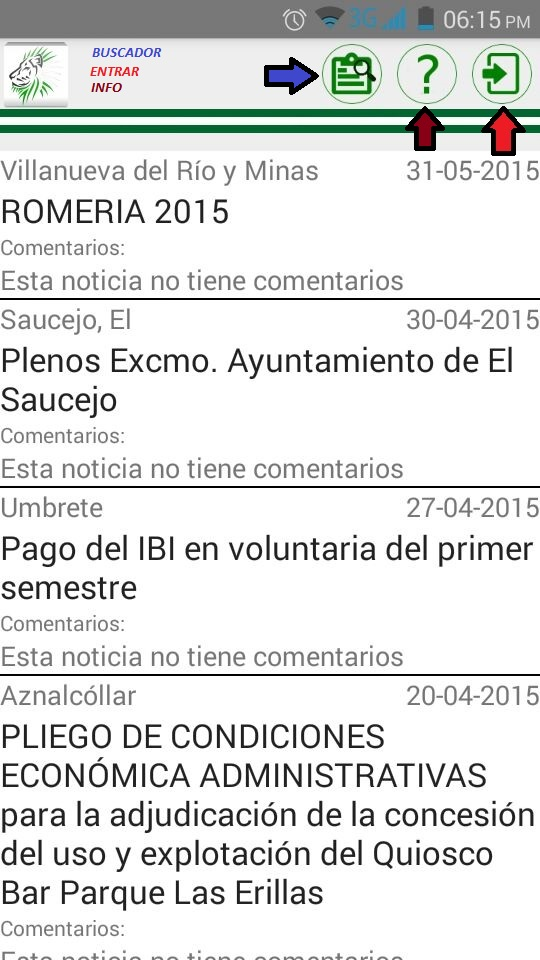
\includegraphics[scale=0.5]{./android/imagenes/botones1.jpg}
\caption{Elementos de navegación deslogueado}
\label{boton1}
\end{figure}

\begin{figure}
\centering
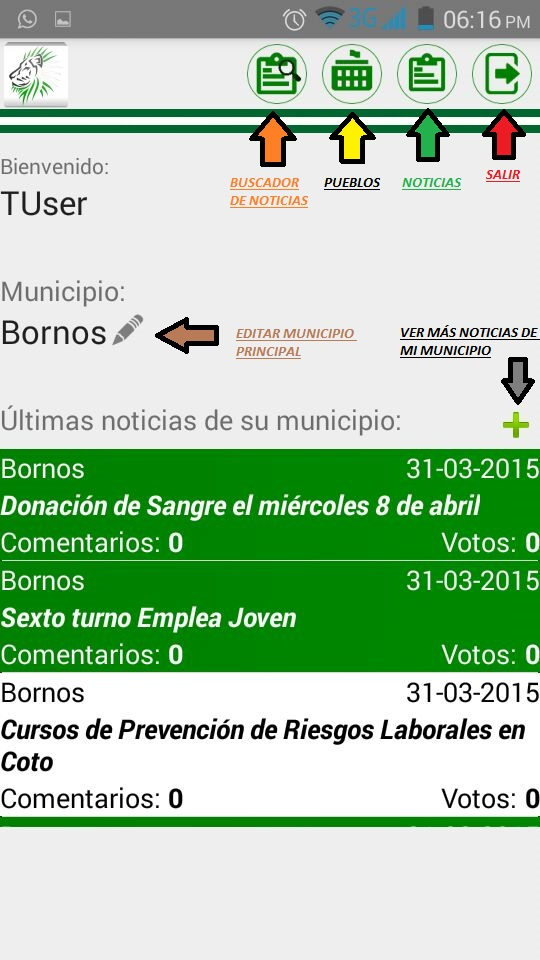
\includegraphics[scale=0.5]{./android/imagenes/botones2.jpg}
\caption{Elementos de navegación logueado}
\label{boton2}
\end{figure}

\begin{figure}
\centering
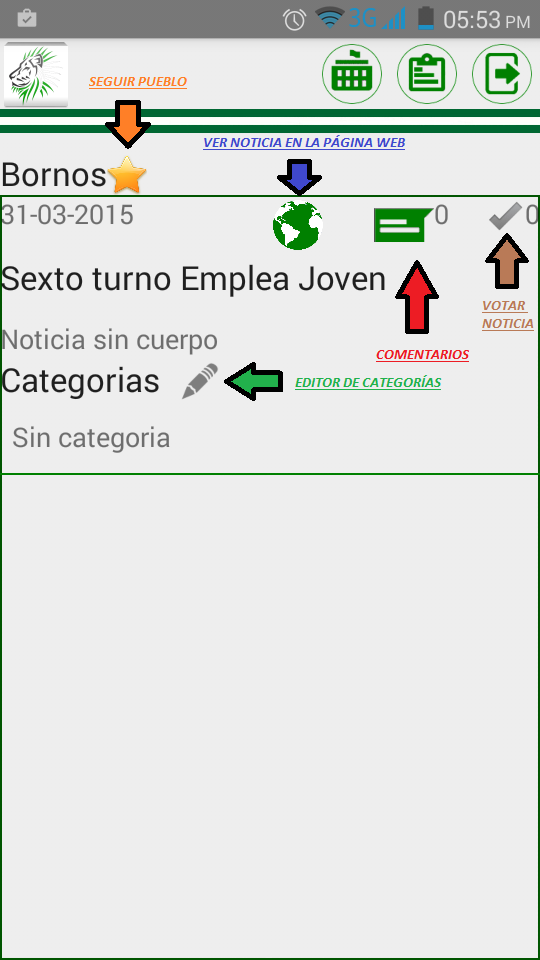
\includegraphics[scale=0.5]{./android/imagenes/botones3.png}
\caption{Otros elementos de navegación}
\label{boton3}
\end{figure}

\begin{figure}
\centering
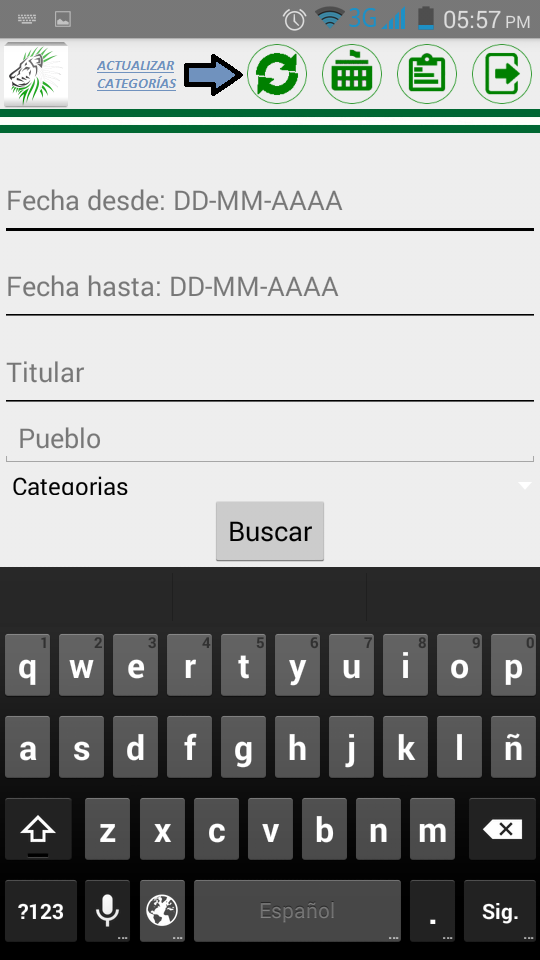
\includegraphics[scale=0.5]{./android/imagenes/botones4.png}
\caption{Actualizar categorias}
\label{boton3}
\end{figure}

\section{Casos de uso}
\subsection{Categorizar noticia}


\begin{figure}
\centering
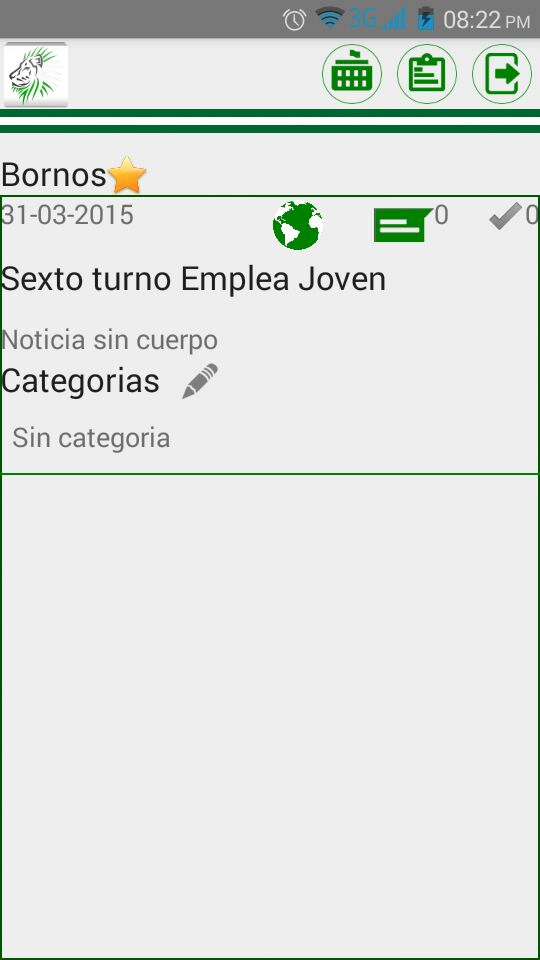
\includegraphics[scale=0.5]{./android/imagenes/cat1.jpg}
\caption{Datos de la noticia}
\label{cat1}
\end{figure}


\begin{figure}
\centering
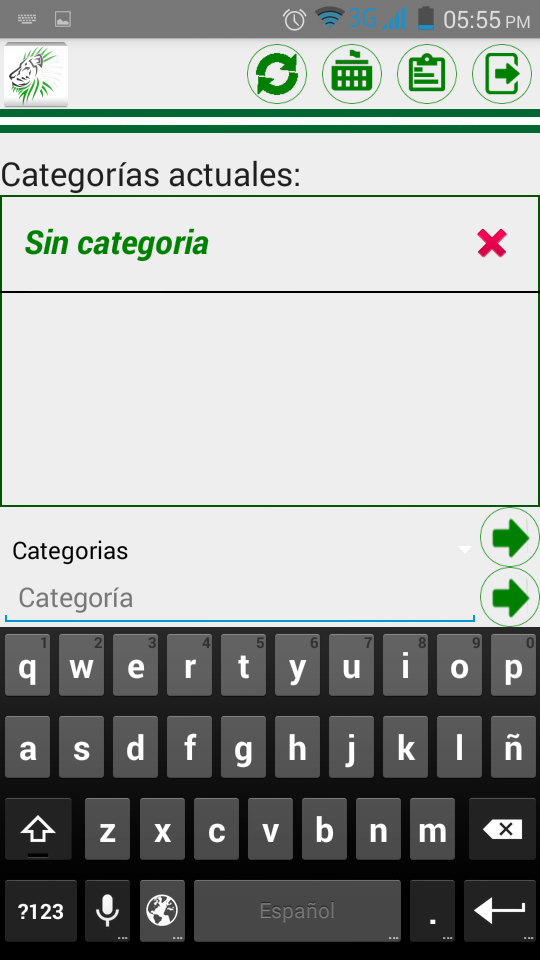
\includegraphics[scale=0.5]{./android/imagenes/cat2.png}
\caption{Listado de categorías}
\label{cat2}
\end{figure}

\begin{figure}
\centering
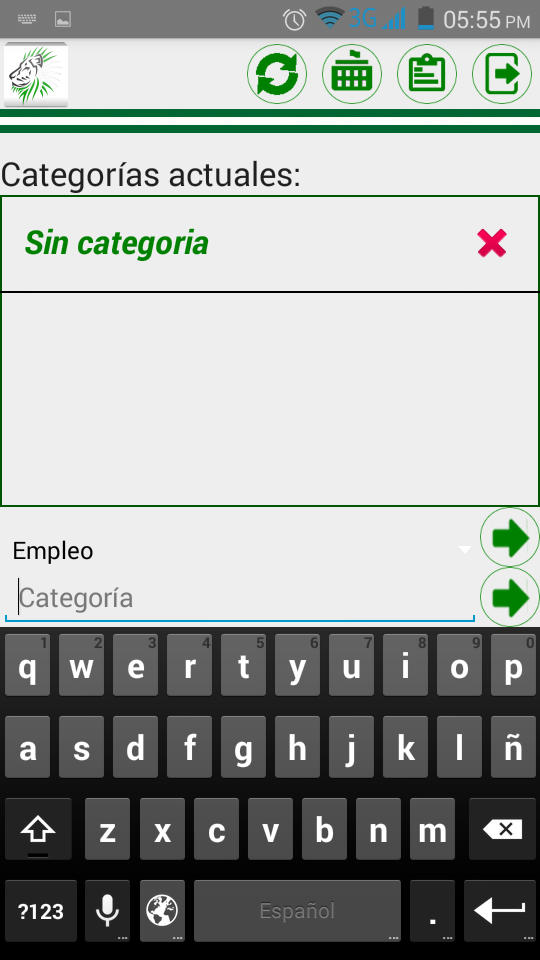
\includegraphics[scale=0.5]{./android/imagenes/cat3.png}
\caption{Agregar categorías ya creadas}
\label{cat3}
\end{figure}

\begin{figure}
\centering
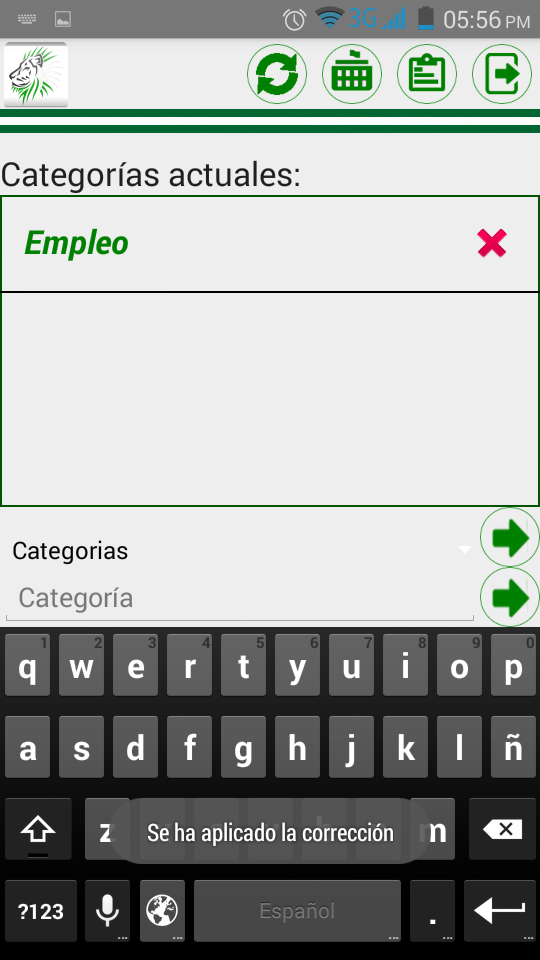
\includegraphics[scale=0.5]{./android/imagenes/cat4.png}
\caption{Comprobación de la agregación de categorías ya creadas}
\label{cat4}
\end{figure}

\begin{figure}
\centering
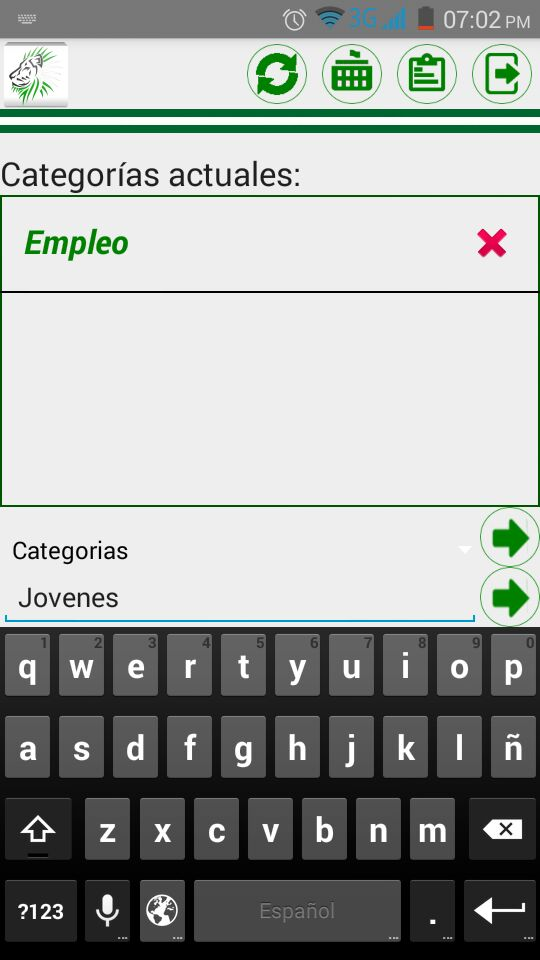
\includegraphics[scale=0.5]{./android/imagenes/cat5.png}
\caption{Agregar una nueva categoría}
\label{cat5}
\end{figure}


\begin{figure}
\centering
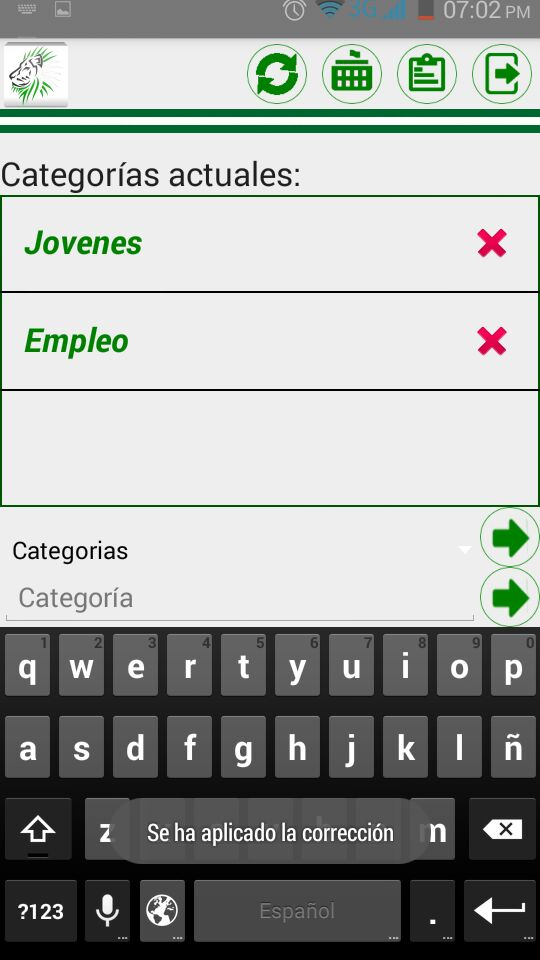
\includegraphics[scale=0.5]{./android/imagenes/cat6.png}
\caption{Comprobación de la agregación de nuevas categorías}
\label{cat6}
\end{figure}

\subsection{Busqueda Noticias}

\begin{figure}
\centering
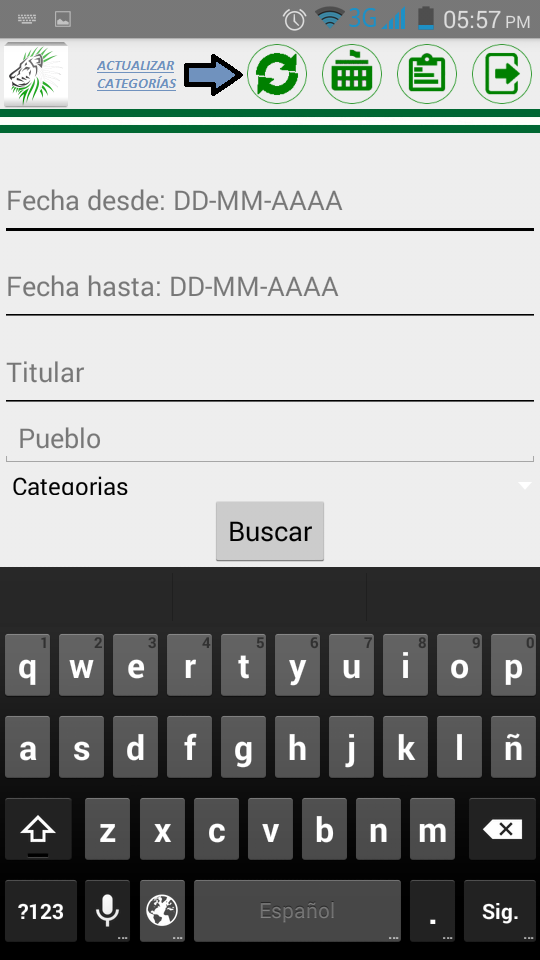
\includegraphics[scale=0.5]{./android/imagenes/bus1.png}
\caption{Acceso a busqueda}
\label{bus1}
\end{figure}

\begin{figure}
\centering
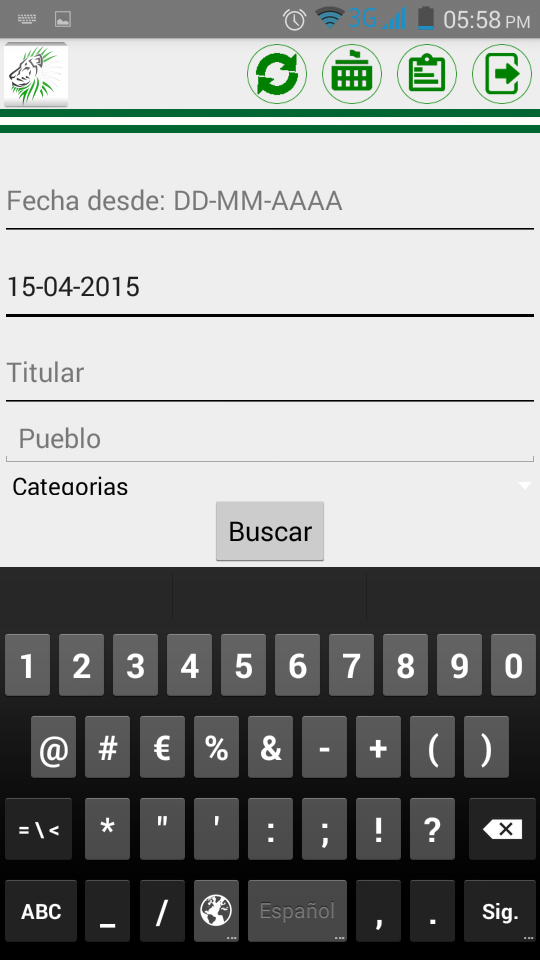
\includegraphics[scale=0.5]{./android/imagenes/bus2.png}
\caption{Relleno de parámetros}
\label{bus2}
\end{figure}

\begin{figure}
\centering

\includegraphics[scale=0.5]{./android/imagenes/bus3.png}
\caption{Resultado}
\label{bus3}
\end{figure}


\subsection{Realizar comentario}

\begin{figure}
\centering
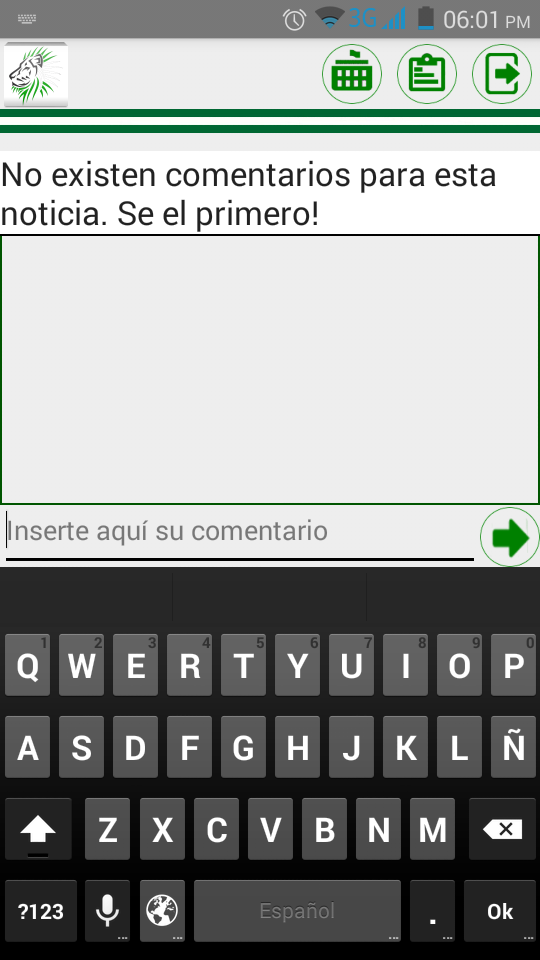
\includegraphics[scale=0.5]{./android/imagenes/com1.png}
\caption{Acceso a Comentarios}
\label{com1}
\end{figure}

\begin{figure}
\centering
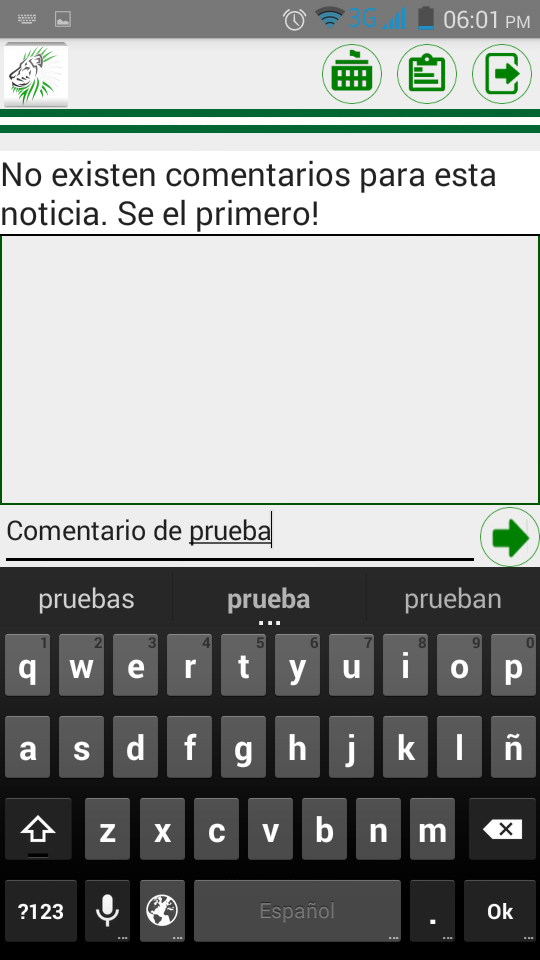
\includegraphics[scale=0.5]{./android/imagenes/com2.png}
\caption{Comentario escrito}
\label{com2}
\end{figure}

\begin{figure}
\centering
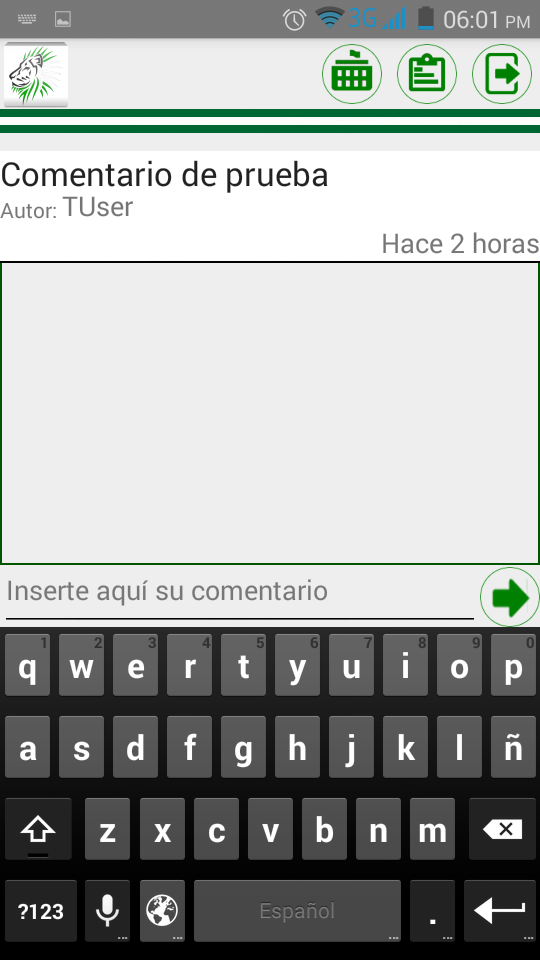
\includegraphics[scale=0.5]{./android/imagenes/com3.png}
\caption{Comentario enviado}
\label{com3}
\end{figure}
%\end{document}

